\documentclass{article}
\usepackage{caption}
\usepackage{subcaption}
\usepackage{graphicx}
\usepackage{tikz}
\usepackage{tikzsymbols}
\usetikzlibrary{calc,patterns,shapes.geometric}
\usepackage{float}

\def\centerarc[#1](#2)(#3:#4:#5){\draw[#1] ($(#2)+({#5*cos(#3)},{#5*sin(#3)})$) arc (#3:#4:#5);}

\pagestyle{empty}
\begin{document}
	\centering
	\begin{figure}[H]
			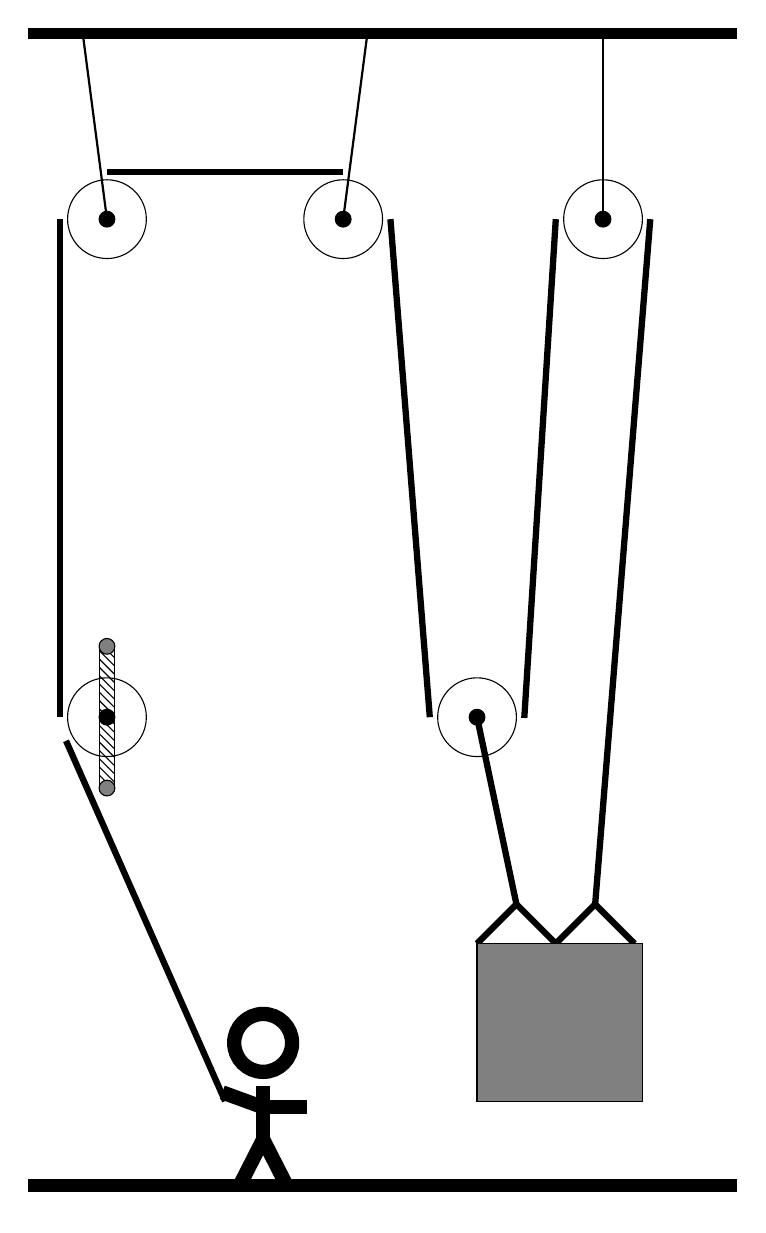
\begin{tikzpicture}
				%%%%% START %%%%%
				\def\a{11.5}
				\def\radlg{0.5}
				\def\radrp{0.6}
				\def\radsm{0.1}
				\def\xone{1}
				\def\yone{\a-0.2*\a}
				\def\xtwo{\xone+3.3}
				\def\ytwo{\a-0.2*\a}
				\def\xthree{\xone+1.7}
				\def\ythree{\a-0.75*\a}
				\def\xh{3.2}
				\def\hlen{\a}
				\def\dx{0}
				\def\dy{-2}
				\def\width{0.8mm}
				\def\ywallone{\yone}
				\def\xwallone{\xone-3}
				\def\ywalltwo{\ythree}
				\def\xwalltwo{\xone-3}
				\def\bump{0.3}
				
				\draw[fill=black] (-3,\a) rectangle (6,\a+0.125);

				\draw (\xone,\yone) circle (\radlg);
				\draw[fill=black] (\xone,\yone) circle (\radsm);
				\draw[thick] (\xone,\yone) -- (\xone+0.3,\a);

				\draw (\xtwo,\ytwo) circle (\radlg);
				\draw[fill=black] (\xtwo,\ytwo) circle (\radsm);
				\draw[thick] (\xtwo,\ytwo) -- (\xtwo,\a);

				\draw (\xthree,\ythree) circle (\radlg);
				\draw[fill=black] (\xthree,\ythree) circle (\radsm);

				\draw[line width=\width]  (\xh-0.5,\a-\hlen) -- (\xh,\a-\hlen+0.5) -- (\xh+0.5,\a-\hlen) -- (\xh+1,\a-\hlen+0.5) -- (\xh+1.5,\a-\hlen);
				\draw[fill=black!50] (\xh-0.5,\a-\hlen) rectangle (\xh+1.6,\a-\hlen-2);			
				
				\draw (\xwallone,\ywallone) circle (\radlg);
				\draw[fill=black] (\xwallone,\ywallone) circle (\radsm);
				\draw[thick] (\xwallone,\ywallone) -- (\xwallone-0.3,\a);
			
				\draw (\xwalltwo,\ywalltwo) circle (\radlg);
				\draw[fill=black] (\xwalltwo,\ywalltwo) circle (\radsm);
				\draw[pattern=north west lines, pattern color=black] (\xwalltwo-0.1,\ywalltwo+\radrp+\bump) rectangle (\xwalltwo+0.1,\ywalltwo-\radrp-\bump); 
				\draw[fill=black!50] (\xwalltwo,\ywalltwo+\radrp+\bump) circle (\radsm);
				\draw[fill=black!50] (\xwalltwo,\ywalltwo-\radrp-\bump) circle (\radsm);
				
				\draw[line width=\width](\dx-0.5,\dy) -- 	({\xwalltwo-\radrp*cos(30)}, {\ywalltwo-\radrp*sin(30)});
				\centerarc[line width=\width](\xwalltwo,\ywalltwo)(180:210:\radrp);
				\draw[line width=\width](\xwalltwo-\radrp, \ywalltwo) -- (\xwallone-\radrp, \ywallone);
				\centerarc[line width=\width](\xwallone,\ywallone)(90:180:\radrp);
				
				\draw[line width=\width](\xwallone, \ywallone+\radrp) -- (\xone,\yone+\radrp);
				\centerarc[line width=\width](\xone,\yone)(0:90:\radrp);
				\draw[line width=\width](\xone+\radrp,\yone) -- (\xthree-\radrp,\ythree);
				\centerarc[line width=\width](\xthree,\ythree)(180:370:\radrp);
				\draw[line width=\width] (\xthree+\radrp,\ythree-0.01) -- (\xtwo-\radrp,\ytwo);
				\centerarc[line width=\width](\xtwo,\ytwo)(0:180:\radrp);
				\draw[line width=\width](\xh+1,\a-\hlen+0.5) -- (\xtwo+\radrp,\ytwo);
				\draw[line width=\width] (\xh,\a-\hlen+0.5) -- (\xthree,\ythree);

				\node at (\dx,\dy) {\Strichmaxerl[10][-20][0]};
						
				\draw[fill=black] (-3,-3) rectangle (6,-3.15);
				%%%%% START %%%%%
			\end{tikzpicture}
	\end{figure}

\end{document}